
\begin{itemize}

\item[1.] Let $V$ be an $n$-dimensional complex vector space and $T : V \rar V$ a linear map.
We say that $v \in V$ is a cyclic vector for $T$ if $\{v, T v, . . . , T^{n-1} v\}$ is a basis for $V$ .
Let $p_T \in \bbc[x]$ and $m_T \in \bbc[x]$ be the characteristic polynomial and the minimal
polynomial of $T$, respectively.
\begin{enumerate}[(a)]
    \item Prove that if $T^{n-1}v \neq 0$ but $T^n v = 0$, then $v$ is a cyclic vector for $T$.
    \begin{proof}

    \end{proof}
    
    \item Prove that if $V$ has a cyclic vector for $T$ then $m_T = p_T$.
    \begin{proof}

    \end{proof}
    
    \item Prove that if $T$ is diagonalizable and $m_T = p_T$, then $V$ has a cyclic vector for $T$.
    \begin{proof}

    \end{proof}
    
    \item Prove that if $V$ has a cyclic vector for $T$ and $S : V \rar V$ is a linear map which commutes with $T$, then $S$ is a polynomial in $T$.
    \begin{proof}

    \end{proof}
\end{enumerate}







\item[2.] Let $V$ and $W$ be real vector spaces, and let $\Hom_{\bbr}(W, V)$ denote the set of linear
transformations $W \rar V$, which is a real vector space.
\begin{enumerate}[(a)]
    \item Let $z \in \bbc$ and $\phi \in \Hom_{\bbr}(\bbc, V)$. Define $z\phi: \bbc \rar V$ by the formula $(z\phi)(w) = \phi(zw)$. Prove that $z \phi \in \Hom_{\bbr}(\bbc, V)$.
    \begin{proof}

    \end{proof}
    
    \item Prove that $\Hom_{\bbr}(\bbc, V)$ is a complex vector space using part (a) to define scalar multiplication.
    \begin{proof}

    \end{proof}
    
    \item Prove that if $d = \text{dim}_{\bbr}(V) < \infty$, then $\text{dim}_{\bbc}(\Hom_{\bbr}(\bbc, V)) = d$.
    \begin{proof}

    \end{proof}
    
    \item Prove that if $f : V \rar W$ is a linear transformation over $\bbr$, then the
function $f^{*} : \Hom_{\bbr}(\bbc, V) \rar \Hom_{\bbr}(\bbc, W)$ defined by $f^{*}(\phi) = f \circ \phi$ is a linear
transformation over $\bbc$.
    \begin{proof}

    \end{proof}
    
    \item Prove that if $\lambda \in \bbr$ is an eigenvalue for a linear transformation $f : V \rar V$, then $\lambda$ is an eigenvalue for $f^{*} : \Hom_{\bbr}(\bbc, V) \rar \Hom_{\bbr}(\bbc, V)$.
    \begin{proof}

    \end{proof}
\end{enumerate}










\item[3.] Let $\sigma : V \rar V$ be any linear map of vector spaces over a field $k$. Define an action
of $k[X]$ on $V$ as follows: for any polynomial $p(X) = \sum{i=0}^{n} c_i X^i \in k[X]$ and any $v \in V$,
$$p(X) \cdot v = p(\sigma)(v) = \sum{i=0}^{n} c_i \sigma^i(v),$$
where $\sigma^0$ is the identity map on $V$ . The kernel of $p(X)$ is defined to be
$$\ker(p(X)) = \{v \in V \ : \ p(X) \cdot v = 0\}.$$
\begin{enumerate}[(a)]
    \item Show that, for any two polynomials $a(X), b(X) \in k[X]$ and any $v \in V$,
    $$a(X) \cdot (b(X) \cdot v) = (a(X)b(X)) \cdot v$$
    \begin{proof}

    \end{proof}
    
    \item Show that $\Kern(p(X))$ is a $\sigma$-invariant subspace of $V$. When $p(X) = X - \lambda$ where $\lambda \in k$, explain why $\Kern(p(X))$ is the eigenspace of $\sigma$ with respect to $\lambda$.
    \begin{proof}

    \end{proof}
    
    \item Let $p(X)$ and $q(X)$ be polynomials in $k[X]$ so that $\text{gcd}(p(X), q(X)) = 1$. Show that 
    $$\Kern(p(X)q(X)) = \Kern(p(X)) + \Kern(q(X))$$
    and that this sum is direct. Further show that, if $c(X) \in k[X]$ is factored as 
    $$c(X) = p_1(X) p_2(X) ... p_m(X)$$
    where $p_i(X) \in k[X]$ and $\text{gcd}(p_i(X), p_j(X)) = 1$ for all $1 \leq i < j \leq m$, then
    $$\Kern(c(X)) = \Kern(p_1(X)) + \Kern(p_2(X)) + ... + \Kern(p_m(X))$$
    and that this sum is direct. (\textbf{Hint}: Use the fact that if $\text{gcd}(p(X), q(X)) = 1$ then there exist $a(X), b(X) \in k[X]$ so that $a(X)p(X) + b(X)q(X) = 1$.)
    \begin{proof}

    \end{proof}
    
    \item Let $\lambda_i \in k$, $1 \leq i \leq t$, be distinct eigenvalues of $\sigma$. Let $B_i = \{u_{ij} : 1 \leq j \leq m_i\}$ be a basis for the eigenspace of $\lambda_i$ for $1 \leq i \leq t$. Use part (c) to show that the union $B_1 \cup B_2 \cup ... \cup B_t$ is a set of independent vectors.
    \begin{proof}

    \end{proof}
\end{enumerate}











\item[4.] For this problem, we let $G$ be a group. If $x, y \in G$, we define the commutator of $x$ and $y$ to be $[x, y] = x^{-1}y^{-1}xy$ and denote the commutator subgroup by $[G, G] = G'$ (recall that the commutator subgroup of $G$ is the subgroup of $G$ that is generated by the commutators of $G$).
\begin{enumerate}[(a)]
    \item Show that the inverse of a commutator is a commutator and that any conjugate of a commutator is a commutator.
    \begin{proof}
    $[x, y]^{-1} = (x^{-1}y^{-1}xy)^{-1} = y^{-1}x^{-1}yx = [y, x]$. Similarly, $z^{-1}[x,y]z = (z^{-1}x^{-1}z) (z^{-1}y^{-1}z) (z^{-1}xz) (z^{-1}yz) = [z^{-1}xz, z^{-1}yz]$.
    \end{proof}
    
    \item Show that $G'$ is a normal subgroup of $G$.
    \begin{proof}
    This was proved above.
    \end{proof}
    
    \item Show that if $\psi \in \text{Aut}(G)$ then $\psi(G')$ is a subgroup of $G'$.
    \begin{proof}
    $\psi([x, y]) = \psi(x^{-1}y^{-1}xy) = \psi(x)^{-1} \psi(y)^{-1} \psi(x) \psi(y)$. Since $\psi \in \text{Aut}(G)$, this takes the form of $u^{-1} v^{-1} u v = [u,v]$.
    \end{proof}
    
    \item Show that if $\phi : G \rar H$ is a homomorphism of groups then $\text{Im}(\phi)$ is abelian if and only if $G'$ is a subgroup of $\Kern(\phi)$.
    \begin{proof}
    $(\Rightarrow)$ Suppose $\text{Im}(\phi)$ is Abelian. Then $\phi([x,y]) = e$, so $G' \subseteq \Kern(\phi)$.

    $(\Leftarrow)$ Suppose $G' \subseteq \Kern(\phi)$. Then $\phi([x,y]) = e$ for all $x,y \in G$, i.e.: $\phi(x) \phi(y) = \phi(y) \phi(x)$.
    \end{proof}
    
    \item Show that if $N$ is a subgroup of $G$ which contains $G'$ then $N$ is a normal subgroup of $G$.
    \begin{proof}
    We know that $G' \vartriangleleft G$, and that $G/G'$ is Abelian. Any subgroup of an Abelian group is normal, so $H/G'$ a subgroup of $G/G'$ implies $H/G' \vartriangleleft G/G'$. Thus by Third Iso. Thm, $H  \vartriangleleft G$.
    \end{proof}
\end{enumerate}








\item[5.] Let $R$ be a commutative ring with identity and $\emptyset \neq S \subseteq R$ be a nonempty subset.
We say that $S$ is \textit{multiplicatively closed} if $s, t \in S \ \Rightarrow \ st \in S$. Additionally, we say
that the set $S$ is \textit{saturated} if $st \in S \ \Rightarrow \ s, t \in S.$
\begin{enumerate}[(a)]
    \item Let $I \subseteq R$ be an ideal. Show that its complement $S := R \setminus I$ is saturated.
    \begin{proof}

    \end{proof}
    
    \item  Let $I \subseteq R$ be an ideal. Show that its complement $S := R \setminus I$ is multiplicatively closed if and only if $R/I$ is an integral domain.
    \begin{proof}

    \end{proof}
    
    \item Suppose that $S$ is a multiplicatively closed subset of $R$ that does not contain 0. Show that there is an ideal in $P \subset R$ that is maximal with respect to the property that $P \cap S = \emptyset$.
    \begin{proof}

    \end{proof}
    
    \item Let $S$ be as in part (c) and suppose that $P$ is maximal with respect to the property that $P \cap S = \emptyset$. Show that $P$ is necessarily prime.
    \begin{proof}

    \end{proof}
\end{enumerate}












\item[6.] In this problem $G$ refers to the group of order 24 whose subgroup lattice appears
below. You must fully justify each answer for full credit.
\begin{center}
    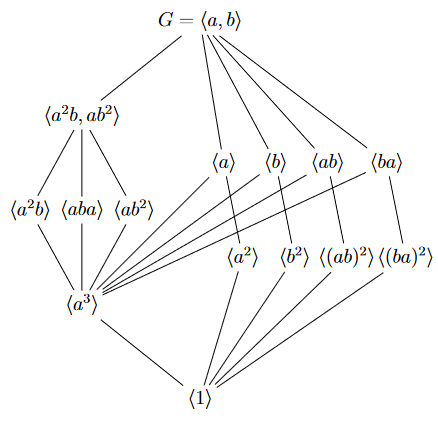
\includegraphics[scale=0.5]{G24.png}
\end{center}

\begin{enumerate}[(a)]
    \item Show that in any group, a subgroup of order 2 is normal if and only if it is contained in the center.
    \begin{proof}

    \end{proof}
    
    \item Partition the fifteen subgroups into equivalence classes by conjugacy.
    \begin{proof}

    \end{proof}
    
    \item Is $G$ is solvable? Nilpotent?
    \begin{proof}

    \end{proof}
    
    \item What familiar group is the quotient $G/\langle a^3 \rangle$ isomorphic to? Justify your answer by drawing its subgroup lattice.
    \begin{proof}

    \end{proof}
    
    \item What familiar group is the subgroup $\ip{a^2 b}{a b^2}$ isomorphic to? Justify your answer by drawing its subgroup lattice.
    \begin{proof}

    \end{proof}
    
    \item What familiar group is the quotient $\ip{a^2 b}{a b^2}/\langle a^3 \rangle$ isomorphic to? Use the isomorphism theorems to justify your answer.
    \begin{proof}

    \end{proof}
\end{enumerate}















\end{itemize}